\section{The ForeC Language}
\label{sec:forec}
Execution platforms have evolved from single-cores to multi-cores. 
Hence, all the synchronous languages designed earlier (e.g., 
Esterel~\cite{timed_esterel}, Lustre~\cite{timed_lustre},  
Signal~\cite{timed_signal}, Esterel C Language~\cite{timed_ecl}, 
Reactive Shared Variables~\cite{timed_reactivec_shared_variables}, 
and \pretc{}~\cite{pret_pretc}) must be remodeled to 
address the challenges raised by multi-cores. Over 30 years of
synchronous programming languages have demonstrated that they
are very well suited to the design of safety-critical real-time
systems~\cite{BriereRPC95,SouyrisPHJBH05}. Moreover, the ideal modeling of 
time brought by the synchrony hypothesis makes them good 
candidates for PRET programming. This motivates our proposed
ForeC language that is dedicated to the programming of multi-cores. 
ForeC inherits the benefits of synchrony, such as determinism
and reactivity, along with the benefits and power of the C language, 
such as control and data structures. This is unlike conventional
synchronous languages, which treat C as an external host language.
A key goal of ForeC is in providing deterministic shared variable
semantics that is agnostic to scheduling. This goal
is essential for the reasoning and debugging of parallel
programs. This section presents ForeC with a 
UAV running example. The formal
semantics of ForeC is then detailed and important proofs
concerning program reactivity and 
determinism~\cite{Maraninchi92,Tardieu07} are provided.

\subsection{Overview and Syntax}
\label{sec:forec:overview}
ForeC is a synchronous language that extends a
safety-critical subset of C~\cite{programming_languages_clight,programming_languages_cyclone} 
(see Section~\ref{sec:introduction:programming_safety}) with a
minimal set of synchronous constructs. We briefly describe the 
statements, type specifiers, and type qualifiers allowed in the C subset:
\begin{description}
	\item[C statements (\emph{c\_st})]
		  Expressions in a statement can only be constants, variables, pointers, and 
		  arrays that are composed with the logical, bitwise, relational, and 
		  arithmetic operators of C. 
		  Although the use of pointers and arrays is allowed, they can make static
		  dataflow analysis difficult~\cite{BussBSE10} because of pointer aliasing. 
		  Thus, we assume that pointers are never reassigned to 
		  point to other variables.
		  All C control statements, except \texttt{goto}, can be used. These are the selection statements 
		  (\texttt{if}--\texttt{else} and \texttt{switch}) and loop statements (\texttt{while}, 
		  \texttt{do}--\texttt{while}, and \texttt{for}).

	\item[C type specifiers] All the C primitives can be used, e.g., \texttt{char}, 
		  \texttt{int}, and \texttt{double}. Custom data types can be defined using
		  \texttt{struct}, \texttt{union}, and \texttt{enum}.

	\item[C type qualifiers (\emph{c\_tq})] All the C \texttt{const}, 
		  \texttt{volatile}, and \texttt{restrict} qualifiers can be used.
		  
	\item[C storage class specifiers] The C \texttt{typedef},
		  \texttt{extern}, \texttt{static}, \texttt{auto}, and \texttt{register} specifiers can be
		  used.
\end{description}

Figure~\ref{fig:forec:syntax} gives
the extended syntax of ForeC and Table~\ref{table:forec:semantics}
summarizes the informal semantics. A statement (\emph{st}) in ForeC
can be a traditional C statement (\emph{c\_st}), or a barrier (\verb$pause$), 
fork/join (\verb$par$), or preemption (\verb$abort$) statement. Using 
the sequence operator (~;~), a statement in ForeC can be an 
arbitrary composition of other statements. Like C, extra
properties can be specified for variables using type
qualifiers. A type qualifier (\emph{tq}) in ForeC is a
traditional C type qualifier (\emph{c\_tq}), an environment
interface (\verb$input$ and \verb$output$), or a
shared variable amongst threads (\verb$shared$). The \verb$input$, 
\verb$output$, and \verb$shared$ type qualifiers precede the 
C type qualifiers in variable declarations. 

\begin{figure}
	\centering
	\begin{tabular}{| l r l |}
		\hline
		\textbf{Statements:}		& \emph{st} & ::= \emph{c\_st} \textbar{} \verb$pause$ \textbar{} \verb$par($\emph{st},~\emph{st}\verb$)$	\\
									&			& ~~~~~\textbar{} \verb$weak$?~\verb$abort$~\emph{st}~\verb$when immediate$?~(\expression{})	\\
									&			& ~~~~~\textbar{} \emph{st}; \emph{st}															\\
									&			&																								\\
		\textbf{Type Qualifiers:}	& \emph{tq}	& ::= \emph{c\_tq} \textbar{} \verb$input$ \textbar{} \verb$output$ \textbar{} \verb$shared$	\\
		\hline
	\end{tabular}
	
	\caption{Syntactic extensions to C.}
	\label{fig:forec:syntax}
\end{figure}

\begin{table}
	\def\arraystretch{1.3}
	
	\tbl{ForeC constructs and their semantics.\label{table:forec:semantics}}{
		\begin{tabular}{| p{\textwidth} |}
			\hline
			\texttt{input}:
				Type qualifier to declare an input, the value of which is updated 
				by the environment at the start of every global tick.						\\ \hline
			\texttt{output}:
				Type qualifier to declare an output, the value of which is emitted 
				to the environment at the end of every global tick.							\\ \hline
			\texttt{shared}:
				Type qualifier to declare a shared variable, which can be accessed by 
				multiple threads.															\\ \hline
			\texttt{pause}:
				Pauses the executing thread until the next global tick.						\\ \hline
			\texttt{par}(\emph{st},~\emph{st}):
				Forks two statements \emph{st} as parallel threads. The 
				\texttt{par} terminates when both threads terminate (join back).			\\ \hline
			\texttt{weak}?~\texttt{abort}~\emph{st}~\texttt{when immediate}?~(\expression{}):
				Preempts its body \emph{st} when the expression \expression{} evaluates to 
				a non-zero value. The optional \texttt{weak} and \texttt{immediate} keywords 
				modify its temporal behavior.												\\
			\hline
		\end{tabular}
	}
\end{table}

\begin{figure}
	\centering
	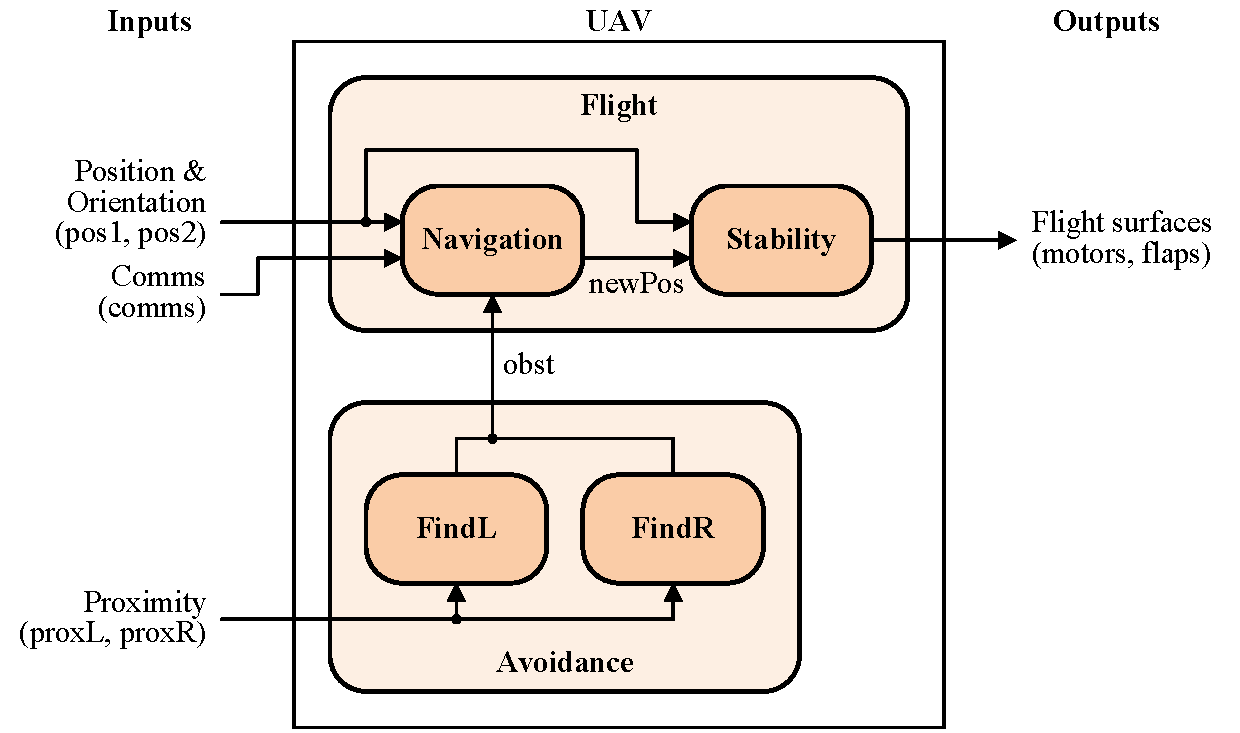
\includegraphics[width=\columnwidth]{images/uav_forec.pdf}

	\caption{Tasks of the UAV.}
	\label{fig:forec:uav_forec}
\end{figure}

As a running example to illustrate the ForeC language, we describe the
design of an unmanned aerial vehicle (UAV) inspired by the
Paparazzi project~\cite{benchmark_papabench}. A UAV is a
remotely controlled aerial vehicle commonly used in
surveillance operations. Figure~\ref{fig:forec:uav_forec} 
presents the functionality of the UAV as a block diagram of tasks. 
The UAV consists of two parallel tasks called \verb$Flight$
and \verb$Avoidance$. The \verb$Flight$ task consists of
two parallel tasks called \verb$Navigation$ and \verb$Stability$.
The \verb$Navigation$ task localizes the UAV with on-board
sensors, updates the flight path, and sends the desired
position to the \verb$Stability$ task. The \verb$Stability$
task controls the flight surfaces to ensure stable flight to
the desired position. The \verb$Avoidance$ task consists of 
two parallel tasks called \verb$FindL$ and \verb$FindR$. 
These tasks use on-board sensors to detect obstacles around 
the UAV and sends collision avoidance data to the 
\verb$Navigation$ task. 

Figure~\ref{fig:forec:uav} is a ForeC implementation of the 
UAV example given in Figure~\ref{fig:forec:uav_forec}.
Figure~\ref{fig:forec:uav_timing1} is a possible execution 
trace of Figure~\ref{fig:forec:uav} to help illustrate the 
execution of ForeC programs. Sections~\ref{sec:introduction:synchronous}
described the execution behavior of synchronous programs. 
To recap, the threads of a synchronous program execute in 
lock-step to the ticking of a \emph{global clock}. In each 
global tick, the threads sample the environment, perform their
computations, and emit their results to the environment.
When a thread completes its computation, we say that it 
has completed its \emph{local tick}. When all the threads complete
their local ticks, we say that the program has completed 
its \emph{global tick}. In Figure~\ref{fig:forec:uav_timing1}, 
the first three global ticks are demarcated along 
the left-hand side. 

\begin{figure}
	\centering
	\begin{minipage}[t]{0.75\columnwidth}
		\lstinputlisting[style=full]{./code/forec/informal/uav.forec}
	\end{minipage}
	\caption{Example ForeC program for the UAV running example.}
	\label{fig:forec:uav}
\end{figure}

\begin{figure}
	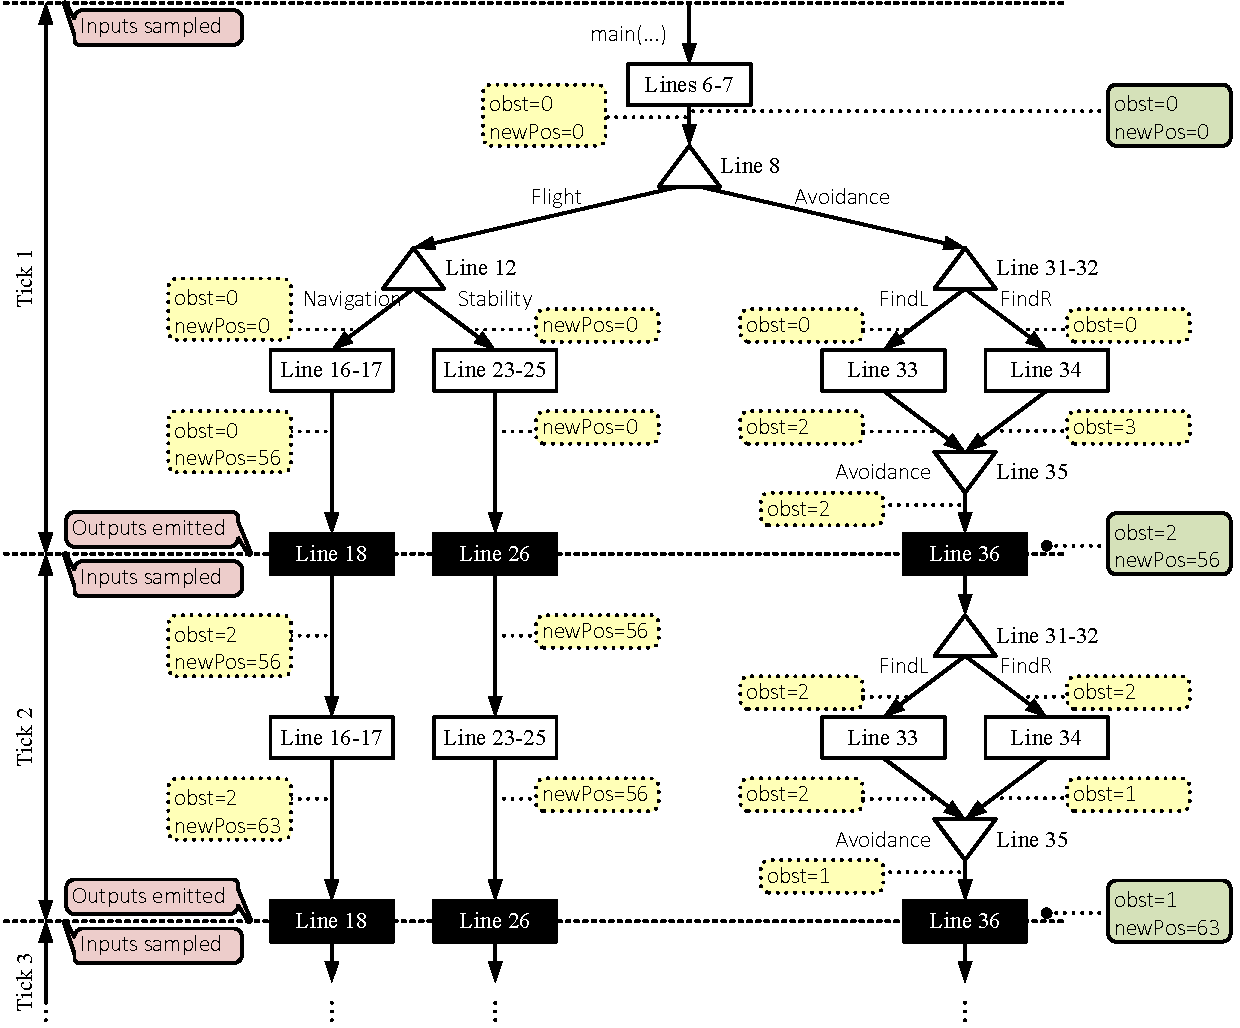
\includegraphics[width=\columnwidth]{images/uav_timing1.pdf}
	\caption{Possible execution trace for Figure~\ref{fig:forec:uav}.}
	\label{fig:forec:uav_timing1}
\end{figure}

In Figure~\ref{fig:forec:uav}, the UAV program starts with 
the inclusion of a C header file (line~\ref{code:forec:uav_header}) 
for the functions used in the 
program and the global variable declarations 
(lines~\ref{code:forec:uav_inputs}--\ref{code:forec:uav_outputs}) to 
interface with the environment. Line~\ref{code:forec:uav_inputs}
declares inputs to capture sensor readings. Inputs
are read-only and their values are updated by the
environment at the start of every global tick. 
Line~\ref{code:forec:uav_outputs} declares outputs
for the actuation commands for the flight motors and
surfaces. Outputs emit their values to the
environment at the end of every global tick. Inputs and
outputs can only be declared in the program's
global scope. The left-hand side of Figure~\ref{fig:forec:uav_timing1}
shows the sampling of inputs and emission of outputs 
at the start and end of each global tick, respectively.

Like traditional C programs, the function \verb$main$ 
(line~\ref{code:forec:uav_main}) is the program's main 
entry point and serves as the initial
thread of execution. Lines~\ref{code:forec:uav_obst}--\ref{code:forec:uav_newpos}
declare variables that can be shared amongst 
threads (see Section~\ref{sec:forec:shared_variables}).
In Figure~\ref{fig:forec:uav_timing1}, the states of 
the shared variables are given inside solid round
boxes at specific points in the execution trace.
Line~\ref{code:forec:uav_obst} declares a shared
variable \verb$obst$ to store the distance and angle 
of the closest obstacle as an encoded integer.
Line~\ref{code:forec:uav_newpos} declares a shared variable
\verb$newPos$ to store the UAV's desired position. 

On line~\ref{code:forec:uav_par1}, the \verb$par$ statement
forks the \verb$Flight$ (line~\ref{code:forec:uav_flight})
and \verb$Avoidance$ (line~\ref{code:forec:uav_avoid})
functions into two parallel \emph{child} threads. We refer
to the threads by their function names, e.g., the
\verb$Flight$ and \verb$Avoidance$ threads. 
The forking of threads is represented in
Figure~\ref{fig:forec:uav_forec} as triangles.
On line~\ref{code:forec:uav_par2}, the \verb$Flight$ thread
forks two more parallel child threads, \verb$Navigation$
(line~\ref{code:forec:uav_nav}) and \verb$Stability$
(line~\ref{code:forec:uav_stability}), creating a hierarchy
of threads. The \verb$par$ statement can also fork blocks of
code, e.g., line~\ref{code:forec:uav_par3} forks the 
\verb$FindL$ and \verb$FindR$ threads. The \verb$par$
is a blocking statement and terminates only when both its
child threads have terminated and joined together. The
joining of threads is represented in
Figure~\ref{fig:forec:uav_timing1} as inverted triangles. 

After the \verb$Navigation$, \verb$Stability$, \verb$FindL$,
and \verb$FindR$ threads have forked, they start executing
their respective body. For example, the \verb$Navigation$
thread enters the \verb$while$-loop
(line~\ref{code:forec:uav_while1}) and computes a new
desired position. Next, the
\verb$pause$ statement \emph{pauses} the thread's execution
(line~\ref{code:forec:uav_pause1}), acting as a
synchronization barrier. In
Figure~\ref{fig:forec:uav_timing1}, the \verb$pause$
statements are shown as black rectangles and the program
completes a global tick when all the threads pause.
This is indicated by the dotted horizontal lines across the
\verb$pause$ statements.

Every time a thread starts its local tick, it creates
\emph{local copies} of all the shared variables that its
body accesses (reads or writes). 
The local copies are initialized at the start of the global tick with
the values that have been resynchronized at the end of the previous
global tick. We use combine functions to compute these resynchronized
values (details below). The shared variables
declared in the program remain distinct from the threads'
local copies. When a thread needs to access a shared
variable, it accesses its local copies instead. Thus, the
changes made by a thread cannot be observed by others,
yielding mutual exclusion and thread isolation. Moreover,
only sequential reasoning is needed within a thread's local
tick. In Figure~\ref{fig:forec:uav_timing1}, the states of a
thread's copies are shown inside dotted round boxes
throughout the execution trace. For example, when the
\verb$Navigation$ thread starts its first local tick, it has
a copy of \verb$obst$ and \verb$newPos$ (values equal to
$0$). When its local tick ends, its copy of \verb$newPos$ 
has been set to $56$.

To enable thread communication, the copies of each shared
variable are automatically \emph{combined} into a single value when the
threads join and when the global tick ends. This is achieved
by a programmer-specified \emph{combine function}. In
Figure~\ref{fig:forec:uav}, the combine function for 
\verb$obst$ (line~\ref{code:forec:uav_obst}) is \verb$min$
(line~\ref{code:forec:uav_min}), specified by the
\verb$combine$ clause, which returns the closest obstacle.
The \verb$combine$ clause also specifies that only the
copies with new values are combined (new since the last global
tick). In global tick one of
Figure~\ref{fig:forec:uav_timing1}, the \verb$FindL$ and
\verb$FindR$ threads set new values ($2$ and $3$) to their
copies of \verb$obst$. When these threads join, the new
values are combined to $2$ and assigned to their parent
thread \verb$Avoidance$. Meanwhile, the \verb$Navigation$
thread only reads its copy of \verb$obst$. Thus, when global
tick one ends, the value of the shared variable \verb$obst$
is set to $2$ by the \texttt{min} function. 
Had there been more copies with new values,
then these copies would have been combined and assigned to
\verb$obst$ before the next global tick started. We say that
the shared variables are \emph{resynchronized} at the end of
each global tick. In Figure~\ref{fig:forec:uav_timing1}, the
resynchronized values are shown inside solid round boxes,
e.g., \texttt{obst} = 2 and \texttt{newPos} = 56. The shared variables start each 
global tick with their resynchronized values. 
For the first global tick only, the resynchronized value of a shared 
variable is its initialization value. 

Appendix~\ref{sec:forec_combine} describes more examples
of combine functions and how more than two
copies are combined. The following sections elaborate on the
details of local and global ticks, fork/join parallelism,
shared variables, and preemption.


%-----------------------------------------------------------------------------

\subsubsection{Local and Global Ticks}
We say that a thread completes its \emph{local tick} when it
pauses, terminates, or forks at least one thread that
completes its local tick without terminating. For example,
in Figure~\ref{fig:forec:uav}, the \verb$Avoidance$ thread 
starts its first local tick 
by forking the child threads \verb$FindL$ and \verb$FindR$
(line~\ref{code:forec:uav_par3}). Assuming that the
\verb$find$ function does not pause, both child threads
complete their local tick by terminating. After the child
threads join, the \verb$Avoidance$ thread reaches a
\verb$pause$ (line~\ref{code:forec:uav_pause2}) and
completes its first local tick. A program completes its
\emph{global tick} when all its threads have completed their
respective local ticks. At the next global tick, the paused
threads start their next local tick from their respective
\verb$pause$s. For brevity, we shorten ``global tick'' into
``tick'' and use ``local tick'' as before.


%-----------------------------------------------------------------------------

\subsubsection{Fork/Join Parallelism}
The \verb$par$ statement enables the forking of parallel
threads. We use the well known terminology related
to parallel programming. The
\emph{parent} thread is the thread that executes the
\verb$par$ statement to fork its \emph{child} threads. The
\emph{parent} thread is also the \emph{ancestor} of its
child threads and their nested child threads. Child threads
forked by the same \verb$par$ statement are \emph{siblings}.
Because the \verb$par$ is a blocking statement, threads
always execute sequentially with respect to their ancestors.
Threads that are not ancestors of each other are
\emph{relatives} and can execute in parallel. 

The thread genealogy of a program can be determined statically by
inspecting the program's control-flow.
Figure~\ref{fig:forec:uav_genealogy_hierarchy} shows the
thread genealogy of the UAV program. Each node is a
thread and arrows are drawn from the children to their
parent thread. Figure~\ref{fig:forec:uav_genealogy_description}
exemplifies the thread genealogy.

\begin{figure}
	\centering

	\subfloat[Thread genealogy.] {
		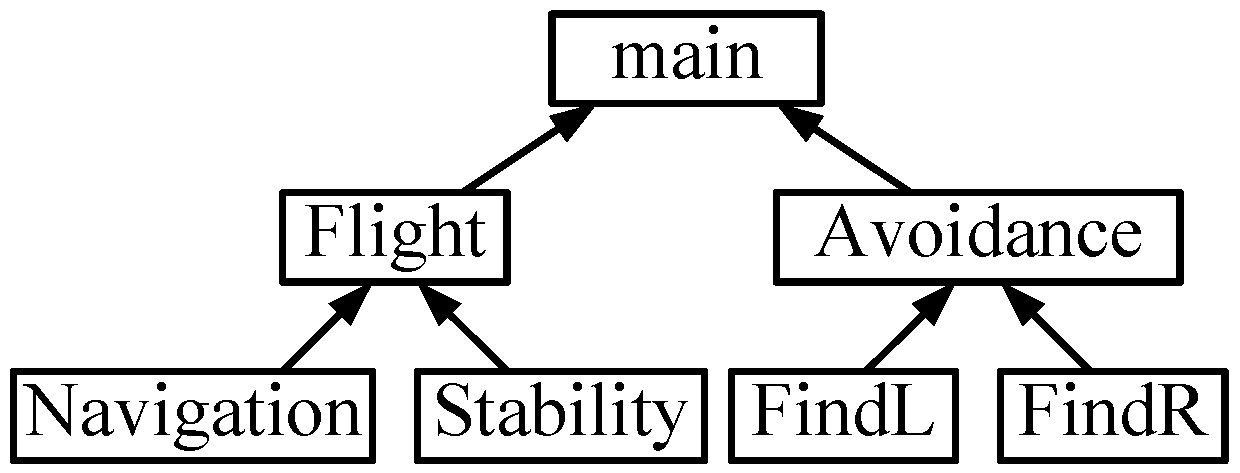
\includegraphics[width=0.4\columnwidth]{uav_genealogy_hierarchy}
		\label{fig:forec:uav_genealogy_hierarchy}
	}
	\hfill
	\subfloat[Descriptive examples.] {
		\begin{minipage}[b]{0.55\textwidth}
			\texttt{main}: Parent of \texttt{Flight} and \texttt{Avoidance}.		\\
			\texttt{Flight}: Parent of \texttt{Navigation} and \texttt{Stability}.	\\
			\texttt{main} and \texttt{Flight}: Ancestors of \texttt{Navigation} and \texttt{Stability}.	\\
			\texttt{FindL} and \texttt{FindR}: Siblings of each other.				\\
			\texttt{Navigation}: Relative of \texttt{Avoidance}, \texttt{FindL}, \texttt{FindR}, and \texttt{Stability}.
		\end{minipage}
		\label{fig:forec:uav_genealogy_description}
	}
	
	\caption{Thread genealogy for Figure~\ref{fig:forec:uav}.}
	\label{fig:forec:uav_genealogy}
\end{figure}


%-----------------------------------------------------------------------------

\subsubsection{Shared Variables}
\label{sec:forec:shared_variables}
All variables in ForeC follow the scoping rules of C. By
default, all variables are \emph{private} and can only be
accessed (read or write) by one thread throughout its scope.
To allow a variable to be accessed by multiple threads, it
must be declared as a \emph{shared} variable by using the
\verb$shared$ type qualifier. Thus, any misuse of private variables are
easy to detect at compile time. Appendix~\ref{sec:forec_combine:passing}
describes how shared variables are passed by value and by reference into
functions. The semantics we propose for 
ForeC makes sure that the shared variables can be safely accessed
by the parallel threads without the need
of mutual exclusion constructs. The goal is to provide a
deterministic shared variable semantics that is agnostic to
scheduling, which is essential for the design and
debug of parallel programs. Within each tick, the accesses
to a shared variable from two threads may occur in sequence or 
in parallel:
\begin{definition}
	\label{def:forec:access_sequential}
	Accesses from two threads are in \emph{sequence} if both 
	threads are not relatives or if the accesses occur in different ticks. 
\end{definition}

\begin{definition}
	\label{def:forec:access_parallel}
	Accesses from two threads are in \emph{parallel} if both 
	threads are relatives and the accesses occur in the same tick.
\end{definition}

Improperly managed parallel accesses to a shared variable
can cause race conditions, leading to non-deterministic 
behavior. For example, two parallel writes to a
shared variable can non-deterministically and partially
overwrite each other's value. A parallel read and write to a
shared variable can result in the read returning the
variable's value before, during, or after the write has
completed. Table~\ref{table:literature:mutual_exclusion} 
in Section~\ref{sec:literature} reviewed 
the solutions that exist for enforcing mutual
exclusion on shared variables, usually by
interleaving parallel accesses into a sequence.
Parallel accesses can be interleaved in many ways
(influenced by the programmer, compiler, and runtime system),
and relying on a particular interleaving for correct program
behavior is brittle and error prone.

%\begin{table}
%	\centering
%
%	\begin{tabular}{| c  c | c | c |}
%		\cline{3-4}
%		\multicolumn{1}{c}{}																& 				& \multicolumn{2}{p{5.8cm} |}{\textbf{Accesses to the shared variable are by relative threads?}}	\\ 
%		\multicolumn{1}{c}{}																& 				& \textbf{Yes}		& \textbf{No}																\\ \cline{1-4}
%		\multirow{2}{6.3cm}{\textbf{Accesses to the shared variable are in the same tick?}}	& \textbf{Yes}	& Parallel Access	&																			\\ \cline{2-3} 
%																							& \textbf{No}	& \multicolumn{2}{c|}{Sequential Access}														\\
%		\hline
%	\end{tabular}
%	\caption{Determining whether two accesses to a shared variable are parallel or sequential.}
%	\label{table:forec:variable_access}
%\end{table}

We propose a shared memory model that permits shared 
variables to be accessed deterministically in parallel, without 
needing the programmer to explicitly use mutual exclusion. 
%PC-MoC is similar in spirit to the sequentially constructive model of 
%computation (SC-MoC)~\cite{timed_seq_concurrency} but targets the 
%execution of synchronous threads on parallel architectures. 
The goals of the model are: 
\begin{description}
	\item[Isolation] Provide isolation between threads to enable the local reasoning of each thread.
		  That is, the execution of a thread's local tick can be understood by only knowing 
		  the values of the variables at the start of the thread's local tick.

	\item[Determinism~\cite{Maraninchi92}] Ensure deterministic execution regardless of scheduling decisions. This guarantees 
		  that deterministic outputs are always generated at the end of each tick.

	\item[Parallelism] Minimize the need to serialize parallel accesses to shared variables. This
		  maximizes the amount of parallel execution that can occur at runtime, which is important 
		  for improving the program's performance.
\end{description}
We propose the following mechanisms for achieving our shared memory model: 
All threads access their own \emph{local copies} of the shared variables, and these 
copies are \emph{resynchronized} every time threads join and when the tick ends.

\subsubsection{Copying of Shared Variables}
\label{sec:forec:shared_variables_copying}
Every time a thread starts its local tick, it creates
\emph{local copies} of all the shared variables that its body
accesses (reads or writes). 
When a thread is forked, its initial copy of a shared variable 
is created from its parent's copy if it exists, otherwise, from 
the shared variable's resynchronized value.
A parent thread that is blocked on a \verb$par$ statement
does not create any copies of the shared variables until 
the \verb$par$ statement terminates. For example, in tick 
two of Figure~\ref{fig:forec:uav_timing1}, the threads 
\texttt{main}, \texttt{Flight}, and \texttt{Avoidance} 
make no local copies. The child threads \texttt{Navigation}, 
\texttt{Stability}, \texttt{FindL}, and \texttt{FindR} must
create their local copies from the shared variables' resynchronized
values, e.g., \texttt{obst}~=~2 and \texttt{newPos}~=~56. 
%Shared variables can be passed as arguments into threads
%(Appendix~\ref{sec:forec_combine:passing}). Following the C
%convention, when a shared variable is \emph{passed by value}, 
%only its value is used to initialize the thread's parameter.
A shared variable declared inside a thread can be shared
among its child threads by \emph{passing a reference} (using a
pointer) into the child threads
(e.g., \verb$obst$ on line~\ref{code:forec:uav_par1} of
Figure~\ref{fig:forec:uav}). When a shared variable is
passed by reference into an ordinary function (e.g.,
\verb$obst$ on line~\ref{code:forec:uav_while2}), the 
function uses the calling thread's copy of the shared variable. 

\subsubsection{Resynchronization of Shared Variables}
\label{sec:forec:shared_variables_resync}
The copies are \emph{resynchronized} every time the program
completes its tick (before outputs are emitted).
Resynchronizing at specific program points ensures that the
semantics of shared variables is agnostic to scheduling. 
We use combine functions to compute the value of resynchronized
shared variables. Combine functions must be
deterministic, associative, and commutative. That
is, the combine function produces the same outputs from the
same inputs, regardless of previous invocations and how the
copies are ordered or grouped. The signature of any combine
function is 
$\mathit{C}: \mathit{Val} \times \mathit{Val} \to \mathit{Val}$. 
The two input parameters are the two
copies to be combined. 
When a \verb$par$ statement terminates, the copies
from the terminating child threads are combined and
assigned to their parent thread's copies of shared variables.
For example, in Figure~\ref{fig:forec:uav_timing1}, the \verb$Avoidance$
thread gets a copy of \verb$obst$ every time \verb$FindL$ and 
\verb$FindR$ terminate. Appendix~\ref{sec:forec_combine} 
describes more examples of combine functions and how more than 
two copies are combined. 

It can be useful to ignore some of the copies when
resynchronizing a shared variable. This is achieved by
specifying a \emph{combine policy} that determines what
copies will be ignored. The combine policies are \verb$new$,
\verb$mod$, and \verb$all$. The combine policy of a shared
variable is specified during variable declaration in the
\verb$combine$ clause, e.g., \verb$combine new with$. The
\verb$new$ policy ignores copies that have the same
value as their shared variable, i.e., which has not changed during 
the tick. 
The \verb$mod$ policy ignores copies that were
not assigned a value during the tick, i.e., have not appeared on
the lefthand side of an assignment.\footnote{This differs 
from the \texttt{new} policy because an assignment 
of the form ``\texttt{x=x}'' will be taken into account by the 
\texttt{mod} policy, but not by the \texttt{new} policy.} The default policy is
\verb$all$ where no copies are ignored. Note that the
combine function is not invoked when only one copy remains.
Instead, that copy becomes the resynchronized value. 
Appendix~\ref{sec:forec_combine} provides extensive 
illustrations comparing the behavior of the combine policies.

%Often, a shared variable is intentionally used where only
%one thread writes to it and the other threads read from it. Its
%combine function would never be invoked if the \verb$new$
%or \verb$mod$ combine policy is used. As a shorthand, the
%\verb$combine$ clause can be dropped from a shared
%variable's declaration if 1) the \verb$new$ or \verb$mod$
%combine policy is used, and 2) it can be statically 
%proved that parallel threads will not write to it. A proof 
%may not always be possible because some writes to the shared 
%variable may be executed conditionally by \verb$if$-statements 
%or loops. The compiler can make the conservative assumption 
%that all conditional writes to a shared will always occur.
%Line~\ref{code:forec:uav_newpos} in
%Figure~\ref{fig:forec:uav} is an example of this
%shorthand.


%-----------------------------------------------------------------------------

\subsubsection{Hierarchical Preemption}
\label{sec:forec:preemption}

\begin{figure}
	\centering
	\footnotesize
	\def\arraystretch{1.3}
	
	\begin{tabular}{| l l l|}
		\hline
		\textbf{Expressions:}	& ~~~\emph{exp}  ::= \emph{val} \textbar{} \emph{var} \textbar{} \emph{ptr}\verb$[$\emph{exp}\verb$]$ \textbar{} \verb$($\emph{exp}\verb$)$ 					& \emph{// Constants, variables, and grouping.}	\\
								&			~~~~~~~~~~\textbar{} \emph{u\_op} \emph{exp} \textbar{} \emph{exp} \emph{b\_op} \emph{exp}															& \emph{// Unary and binary expressions.}		\\
		\textbf{Unary}			&																																								&												\\
		\textbf{Operators:}		& \emph{u\_op}	 ::= \verb$*$ \textbar{} \verb$&$ \textbar{} \verb$!$ \textbar{} \verb$-$ \textbar{} \verb$~$										 			& \emph{// Indirection, address, negation,}		\\
								&																																								& \emph{~~~~~~~negative, and one's complement.}	\\
		\textbf{Binary}			&																																								&												\\
		\textbf{Operators:}		& \emph{b\_op}	 ::= \verb$||$ \textbar{} \verb$&&$ \textbar{} \verb$^$ \textbar{} \verb$|$ \textbar{} \verb$&$ \textbar{} \verb$<<$ \textbar{} \verb$>>$ 		& \emph{// Logical and bitwise operators.}		\\
								&			~~~~~~~~~~\textbar{} \verb$==$ \textbar{} \verb$!=$ \textbar{} \verb$<$ \textbar{} \verb$>$ \textbar{} \verb$<=$ \textbar{} \verb$>=$				& \emph{// Relational operators.}				\\
								&			~~~~~~~~~~\textbar{} \verb$+$ \textbar{} \verb$-$ \textbar{} \verb$*$ \textbar{} \verb$/$ \textbar{} \verb$%$										& \emph{// Arithmetic operators.}				\\
		\hline
	\end{tabular}
	
	\caption{Syntax of preemption conditions.}
	\label{fig:forec:abort_expressions}
\end{figure}

\begin{figure}
	\centering

	\begin{minipage}[t]{0.67\columnwidth}
		\lstinputlisting[style=full]{./code/forec/informal/uav_abort.forec}
	\end{minipage}

	\caption{Figure~\ref{fig:forec:uav} extended with preemption.}
	\label{fig:forec:uav_abort}
\end{figure}

\begin{figure}
	\centering

	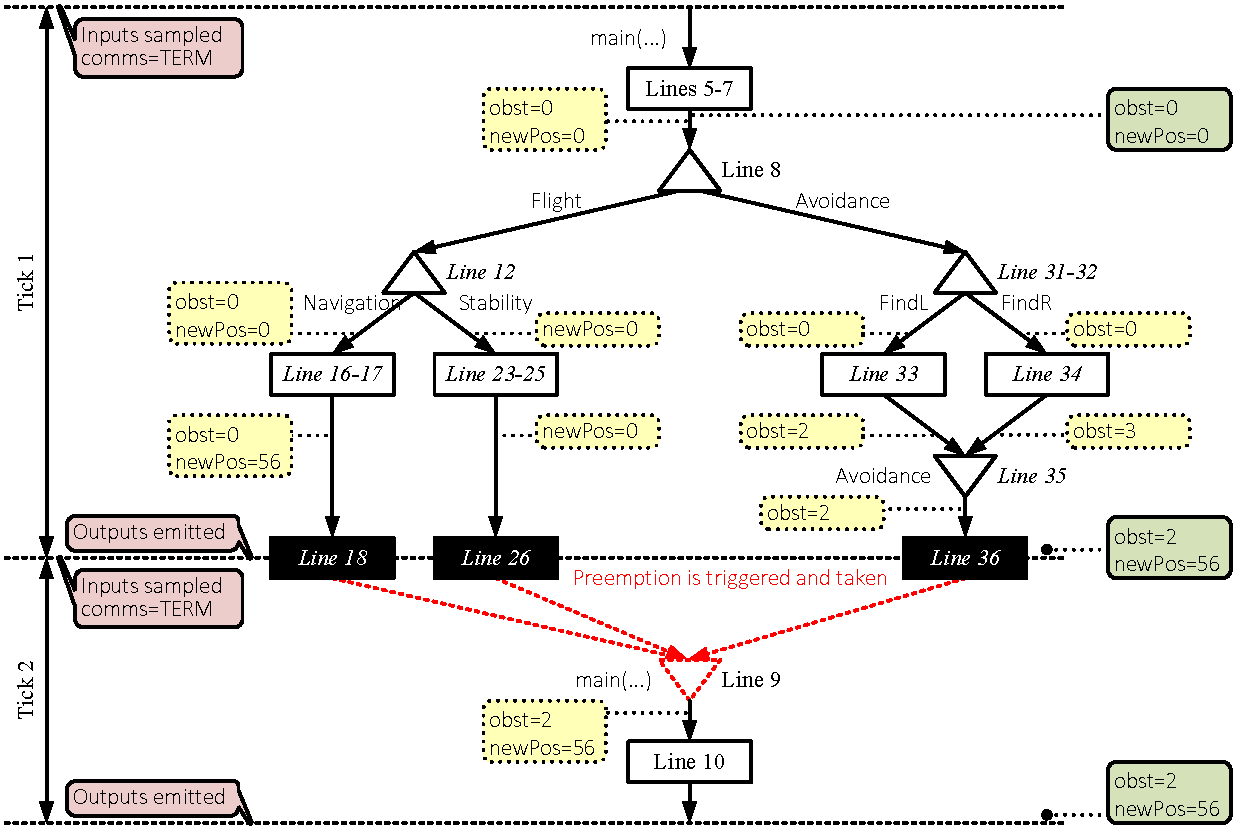
\includegraphics[width=\columnwidth]{images/uav_timing2.pdf}

	\caption{Possible execution trace for Figure~\ref{fig:forec:uav_abort}.}
	\label{fig:forec:uav_timing2}
\end{figure}

Inspired by Esterel~\cite{timed_esterel}, the
\verb$abort$~\emph{st} \verb$when$~(\expression{}) statement
provides preemption~\cite{timed_preemption}, which is the
termination of the \verb$abort$ body \emph{st} when the
condition \expression{} evaluates to \emph{true}. Preemption
can be used to model state machines succinctly. The
condition \expression{} must be a side-effect free
expression produced from the syntax shown 
in Figure~\ref{fig:forec:abort_expressions}. 
In Figure~\ref{fig:forec:uav_abort},
the \verb$main$ function of the UAV has been extended to
respond to external commands through the input 
\verb$comms$ (line~\ref{code:forec:uav_abort_comms}). 
The value of \verb$comms$ can be \verb$OK$, \verb$ERROR$, 
\verb$WARN$, or \verb$TERM$ (line~\ref{code:forec:uav_abort_state}).
The \verb$abort$ statement on
line~\ref{code:forec:uav_abort_abort} preempts the 
execution of all the UAV tasks when \verb$TERM$
is received. A possible execution trace of the 
program of Figure~\ref{fig:forec:uav_abort} is given in
Figure~\ref{fig:forec:uav_timing2}. The \emph{italicized}
line numbers in Figure~\ref{fig:forec:uav_timing2} refer 
to the line numbers in Figure~\ref{fig:forec:uav}, while 
the non-italicized line numbers refer to the line numbers in 
Figure~\ref{fig:forec:uav_abort}. We now explain the semantics of
the \verb$abort$ statement. The preemption of the
\verb$abort$ must be \emph{triggered} before the \verb$abort$
body can be terminated. Preemption is never taken when the
\verb$abort$ body executes for the first time (e.g., tick
one in Figure~\ref{fig:forec:uav_timing2}). At the start of
each subsequent tick, the condition \expression{} is
evaluated before the \verb$abort$ body can execute. This
allows shared variables in the condition to be evaluated
with their resynchronized value. If \expression{} 
evaluates to \emph{true} (any non-zero value following the C
convention), then the preemption is triggered and the
\verb$abort$ statement is terminated. At the start of tick
two in Figure~\ref{fig:forec:uav_timing2}, preemption is
triggered because the preemption condition evaluates to \emph{true}.
The \verb$abort$ statement also terminates if its body
terminates normally. 

Preemptions in ForeC differ from those in Esterel because
Esterel uses signals for thread communication rather than 
shared variables. As explained in
Section~\ref{sec:introduction:synchronous}, signals in
Esterel are either present or absent in each tick and this
information is propagated instantaneously among the threads
without delay. Thus, preemptions in Esterel are triggered
instantaneously, whereas preemptions in ForeC are triggered
with a delay of one tick because the condition 
\expression{} is evaluated using values computed 
in the previous tick. Like
Esterel~\cite{timed_preemption}, the optional \verb$weak$
and \verb$immediate$ keywords change the temporal behavior
of preemptions. The \texttt{weak} keyword delays the
termination of the \texttt{abort} body until the body
cannot execute any further, e.g., reaches a \texttt{pause}
statement. The \texttt{immediate} keyword allows preemption to be
triggered immediately when execution reaches the 
\texttt{abort} for the first time. That is, the preemption condition
\expression{} is evaluated immediately when execution
reaches the \texttt{abort}. This is similar to Esterel's
\texttt{immediate} \texttt{abort} behavior.
To illustrate these four different preemption 
behaviors, Figure~\ref{fig:forec:aborts_abort} 
presents an \texttt{abort} with the optional keywords commented out. 
\begin{description}
	\item[Non-immediate and strong \texttt{abort}] The \texttt{weak} and 
		  \texttt{immediate} keywords are commented out in 
		  Figure~\ref{fig:forec:aborts_abort}. This gives the default preemption
		  behavior, summarized in Figure~\ref{fig:forec:aborts_strong}.
		  In tick one, the
		  \texttt{main} thread sets its copy of \texttt{s} to 1 and prints
		  ``1''. Next, the threads \texttt{t0} and \texttt{t1} set their
		  copies of \texttt{s} to 2 and 5, respectively. When the tick
		  ends, using the combine policy \texttt{all}, the
		  resynchronized value of \texttt{s} is 7. In tick two, the
		  \texttt{abort}'s preemption is triggered and the \texttt{abort}
		  body is terminated, resulting in ``7'' being printed. 
	
	\item[Non-immediate and weak \texttt{abort}] Only the \texttt{weak} 
		  keyword is uncommented in Figure~\ref{fig:forec:aborts_abort}.
		  Figure~\ref{fig:forec:aborts_weak} summarizes the preemption
		  behavior. The execution of tick one proceeds identically to 
		  the non-immediate and strong \texttt{abort} variant. In tick two, 
		  the \texttt{abort}'s preemption is triggered. However, the termination
		  of the \texttt{abort} body is delayed until threads \texttt{t0} and 
		  \texttt{t1} complete their local ticks.
		  This allows \texttt{t0} and \texttt{t1} to set their copies 
		  of \texttt{s} to 3 and 6, respectively. Thus, ``9''
		  is printed.
	
	\item[Immediate and strong \texttt{abort}] Only the \texttt{immediate} 
		  keyword is uncommented in Figure~\ref{fig:forec:aborts_abort}.
		  Figure~\ref{fig:forec:aborts_immediate} summarizes the 
		  preemption behavior. In tick one, the \texttt{main} thread sets
		  its copy of \texttt{s} to 1 and prints ``1''. Next, the
		  \texttt{abort}'s preemption condition is evaluated immediately.
		  Intuitively, because ``1'' was printed for the value of 
		  \texttt{s}, the condition \texttt{s>0} should
		  evaluate to \emph{true}. The counter-intuitive result of 
		  \emph{false} would occur if the resynchronized value of \texttt{s} 
		  was used. Thus, when execution reaches an immediate
		  \texttt{abort}, the condition \expression{} is evaluated 
		  immediately with the thread's copies of the shared variables. 
		  In subsequent ticks, the resynchronized values of the shared 
		  variables are used. In tick one of Figure~\ref{fig:forec:aborts_immediate}, 
		  because the preemption has been triggered, the 
		  \texttt{abort} body is terminated without executing.
	
	\item[Immediate and weak \texttt{abort}] Both the \texttt{weak} and
		  \texttt{immediate} keywords are uncommented in 
		  Figure~\ref{fig:forec:aborts_abort}. 
		  Figure~\ref{fig:forec:aborts_immediate_weak} summarizes the
		  preemption behavior. In tick one, the \texttt{main} thread sets
		  its copy of \texttt{s} to 1 and prints ``1''. Next, the
		  \texttt{abort}'s preemption is triggered immediately. However,
		  the termination of the \texttt{abort} body is delayed until 
		  threads \texttt{t0} and \texttt{t1} complete their local ticks.
		  This allows \texttt{t0} and 
		  \texttt{t1} to set their copies of \texttt{s} to 2 and 5, respectively.
		  Hence, ``7'' is printed.
\end{description}

\begin{figure}
	\centering
	
	\subfloat[Example code.] {
		\begin{minipage}[b]{0.6\textwidth}
			\lstinputlisting[style=full]{./code/forec/informal/abort.forec}
		\end{minipage}
		\label{fig:forec:aborts_abort}
	}
	
	\subfloat[Non-immediate and strong \texttt{abort}.] {
		\footnotesize
		\def\arraystretch{1.3}
		\begin{tabular}{| p{0.4\textwidth} |}
			\hline
			{\bf Tick 1:}	``1'' printed.										
							\texttt{s} = \texttt{plus}(2,5) = 7.				\\ \hline
			{\bf Tick 2:}	Preemption is triggered and the						
							\texttt{abort} body is terminated.					
							``7'' printed.										\\
																				\\
			\hline
		\end{tabular}
		\label{fig:forec:aborts_strong}
	}
	\hfill
	\subfloat[Non-immediate and weak \texttt{abort}.] {
		\footnotesize
		\def\arraystretch{1.3}
		\begin{tabular}{| p{0.4\textwidth} |}
			\hline
			{\bf Tick 1:}	``1'' printed.										
							\texttt{s} = \texttt{plus}(2,5) = 7.				\\ \hline
			{\bf Tick 2:}	Preemption is triggered. 							\\
							\texttt{s} = \texttt{plus}(3,6) = 9.				
							The \texttt{abort} body is terminated. ``9'' printed.\\ 
			\hline
		\end{tabular}
		\label{fig:forec:aborts_weak}
	}

	\subfloat[Immediate and strong \texttt{abort}.] {
		\footnotesize
		\def\arraystretch{1.3}
		\begin{tabular}{| p{0.4\textwidth} |}
			\hline
			{\bf Tick 1:}	``1'' printed. Preemption is						
							triggered and the \texttt{abort} body is terminated.
							``1'' printed again.								\\
			\hline
		\end{tabular}
		\label{fig:forec:aborts_immediate}
	}
	\hfill
	\subfloat[Immediate and weak \texttt{abort}.] {
		\footnotesize
		\def\arraystretch{1.3}
		\begin{tabular}{| p{0.4\textwidth} |}
			\hline
			{\bf Tick 1:}	``1'' printed. Preemption is							
							triggered. \texttt{s} = \texttt{plus}(2,5) = 7.	
							The \texttt{abort} body is terminated. ``7'' printed.\\
			\hline
		\end{tabular}
		\label{fig:forec:aborts_immediate_weak}
	}

	\caption{Abort variants.}
	\label{fig:forec:aborts}
\end{figure}

%For weak aborts, we choose not to check the preemption 
%after the abort body cannot execute any further. 
%This is because, if the preemption
%condition has shared variables, all the nested threads 
%would have to finish executing first before the values of
%the shared variables can be resolved to check the preemption
%condition. This would severely reduce the program's parallelism.
%In addition, for two nested weak abort statement with the
%same preemption condition, the outer condition can evaluate
%to a different value than the inner condition. The execution
%of code between the checking of the preemption conditions
%can change the state of the variables.

%If a statement should only be executed after an \verb$abort$ 
%has preempted, then the 
%``\verb$weak$?~\verb$abort$~$st_0$~\verb$when immediate$?~(\expression{})~\verb$do$~$st_1$''
%variant should be used. The statement $st_1$ in the 
%``\verb$do$~$st_1$'' clause is only after a preemption is taken. 
%If the body terminates 
%normally, then $st_1$ is not executed. This allows
%$st_1$ to be used to implement \emph{cleanup} code.
%This \verb$abort-do$ variant can be structurally translated into an 
%ordinary \verb$abort$:
%\begin{lstlisting}[style=snippet]
%int preempted=0;
%weak? abort st(*$_1$*) when immediate? (preempted=exp);
%if (preempted) {st(*$_2$*);}
%\end{lstlisting}
%where \verb$preempted$ is a uniquely defined variable.

\begin{figure}
	\centering

	\begin{minipage}[t]{0.65\columnwidth}
		\lstinputlisting[style=full]{./code/forec/informal/aborts_nested.forec}
	\end{minipage}

	\caption{Nesting of preemptions.}
	\label{fig:forec:aborts_nested}
\end{figure}

The \verb$abort$ statements can be nested to create 
a hierarchy of preemptions with the outer abort executing 
before the inner aborts. Thus, the preemption 
behavior of the outer \verb$abort$ takes precedence 
over the inner \verb$abort$s. Figure~\ref{fig:forec:aborts_nested}
is an example of an immediate and weak
\verb$abort$ (line~\ref{code:forec:aborts_nested_outer}) 
with a nested immediate and strong \verb$abort$
(line~\ref{code:forec:aborts_nested_inner}).
In tick one, preemption is triggered for the outer
weak \verb$abort$. The variable \verb$x$ is set to 2
and the inner strong \verb$abort$ preempts
immediately without executing its body. Next, \verb$x$ is set to 5 and the 
outer weak \verb$abort$ takes its preemption when 
it reaches the \verb$pause$ on line~\ref{code:forec:aborts_nested_pause}. 
Finally, ``5'' is printed.


%-----------------------------------------------------------------------------

\subsubsection{Bounded Loops}
\label{sec:forec:programming}
In addition to the strict C-coding guidelines described in 
Section~\ref{sec:introduction:programming_safety}, 
ForeC forbids the use of \emph{unbounded recursion} of function calls and 
thread forking to ensure static WCRT analyzability. 
The synchrony hypothesis requires each tick to execute 
in finite time, which means that all statements 
need to have bounded execution times. Unfortunately, loop constructs 
(\verb$for$ and \verb$while$) can have unbounded iterations, leading to
unbounded execution times. Thus, if a loop construct is used, 
then the programmer must guarantee that it always terminates or executes
a \verb$pause$ in each iteration. 
Guaranteeing that a loop always executes a \verb$pause$ may not be 
possible when \verb$pause$ statements are enclosed by \verb$if$-statements. 
The compiler makes conservative assumptions to prove whether 
a loop always executes a \verb$pause$ in each iteration. For example, 
a loop is assumed to always execute a \verb$pause$ in each iteration if 
its body has at least one statement that always executes a \verb$pause$. 
An \verb$if$-statement is assumed to always execute a \verb$pause$ if both 
its branches always execute a \verb$pause$. An 
\verb$abort$ statement is assumed to never execute a \verb$pause$. A 
\verb$par$ statement is assumed to always execute a \verb$pause$ if at 
least one of its child threads always executes a \verb$pause$. The compiler
can perform structural induction on the program's control-flow to conservatively 
prove whether every loop in the program will always execute a \verb$pause$ 
in each iteration.

\begin{table}
	\centering
	\def\arraystretch{1.3}
	
	\tbl{Structural translations of bounded loops.\label{table:forec:loop_translations}}{
		\begin{tabular}{| l | l |}
			\hline
			\textbf{Bounded Loop}					& \textbf{Translation}													\\ 
			\hline
			\texttt{for (init; cond; update) \#n \{st\}}	& \texttt{int cnt=0;}											\\
															& \texttt{for (init; cond \&\& (cnt<n); (update,cnt++)) \{st\}}	\\ \hline
			\texttt{while (cond) \#n \{st\}}				& \texttt{for ( ; cond;) \#n \{st\}}							\\ \hline
			\texttt{do \{st\} while (cond) \#n}				& \texttt{int first=1;}											\\
															& \texttt{for ( ; cond \&\& (first==0); first=0) \#n \{st\}}	\\ \hline
		\end{tabular}
	}
\end{table}


Inspired by \pretc{}~\cite{pret_pretc}, 
we have extended the syntax of loops to also allow 
the programmer to write 
bounded loops, shown in the first column of Table~\ref{table:forec:loop_translations}. 
The ``\verb$#n$'' after the loop header specifies 
that only up to \verb$n$ iterations can be executed.
The second column of Table~\ref{table:forec:loop_translations}
gives the structural translation of bounded loops. 
%For the translation of a bounded \verb$for$-loop,
%the variable \verb$cnt$ tracks the number of iterations that have 
%executed. The condition \verb$(cnt<n)$ guarantees that 
%only up to \verb$n$ iterations are executed. The bounded 
%\verb$while$-loop is translated into a bounded \verb$for$-loop. 
%For the translation of a bounded \verb$do$--\verb$while$-loop, 
%the variable \verb$first$ is used to delay the evaluation of 
%\verb$cond$ to the second iteration. This delay emulates the 
%execution behavior of a \verb$do$--\verb$while$-loop. 
